% Grafo de ε-vecindad
% Compilar con: pdflatex epsilon_neighborhood_graph.tex
\documentclass[tikz,border=10pt]{standalone}
\usepackage{tikz}
\usepackage{xcolor}
\definecolor{gdlblue}{RGB}{41, 98, 168}
\definecolor{gdlred}{RGB}{191, 49, 49}
\definecolor{gdlgreen}{RGB}{30, 130, 76}
\definecolor{gdlorange}{RGB}{217, 130, 30}
\definecolor{gdlpurple}{RGB}{118, 56, 138}
\definecolor{gdlgray}{RGB}{140, 140, 140}
\definecolor{gdlyellow}{RGB}{190, 140, 10}
\usetikzlibrary{decorations.pathmorphing, calc, backgrounds}

\begin{document}
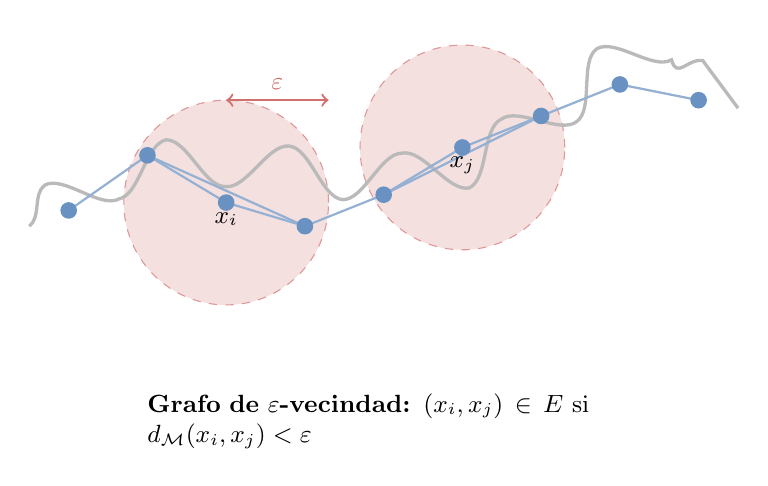
\begin{tikzpicture}[
    point/.style={circle, fill=gdlblue!70, minimum size=6pt, inner sep=0pt},
    edge/.style={thick, draw=gdlblue!50},
    epsilon/.style={dashed, draw=gdlred!50, fill=gdlred!15}
]

% Curva suave representando la variedad
\draw[very thick, gdlgray!60, decorate, decoration={snake, amplitude=0.3cm, segment length=1.5cm}]
    (-4,-0.5) .. controls (-2,1) and (0,-1) .. (2,0.5) .. controls (4,2) .. (5,1);

% Puntos muestreados en la variedad
\coordinate (p1) at (-3.5, -0.3);
\coordinate (p2) at (-2.5, 0.4);
\coordinate (p3) at (-1.5, -0.2);
\coordinate (p4) at (-0.5, -0.5);
\coordinate (p5) at (0.5, -0.1);
\coordinate (p6) at (1.5, 0.5);
\coordinate (p7) at (2.5, 0.9);
\coordinate (p8) at (3.5, 1.3);
\coordinate (p9) at (4.5, 1.1);

% Círculos ε alrededor de algunos puntos
\begin{scope}[on background layer]
    \draw[epsilon] (p3) circle (1.3cm);
    \draw[epsilon] (p6) circle (1.3cm);
\end{scope}

% Aristas del grafo (conexiones dentro de ε)
\draw[edge] (p1) -- (p2);
\draw[edge] (p2) -- (p3);
\draw[edge] (p3) -- (p4);
\draw[edge] (p4) -- (p5);
\draw[edge] (p5) -- (p6);
\draw[edge] (p6) -- (p7);
\draw[edge] (p7) -- (p8);
\draw[edge] (p8) -- (p9);

% Conexiones adicionales por proximidad
\draw[edge] (p2) -- (p4);
\draw[edge] (p5) -- (p7);

% Nodos (puntos)
\foreach \p in {p1,p2,p3,p4,p5,p6,p7,p8,p9} {
    \node[point] at (\p) {};
}

% Etiquetas
\node[below, font=\small] at (p3) {$x_i$};
\node[below, font=\small] at (p6) {$x_j$};

% Flecha de ε
\draw[<->, thick, gdlred!70] ($(p3) + (0, 1.3)$) -- node[above, font=\small] {$\varepsilon$} ($(p3) + (1.3, 1.3)$);

% Leyenda
\node[font=\small, text width=6cm, below] at (0.5, -2.5) {
    \textbf{Grafo de $\varepsilon$-vecindad:} $(x_i, x_j) \in E$ si $d_{\mathcal{M}}(x_i, x_j) < \varepsilon$
};

\end{tikzpicture}
\end{document}
